\Huge\textbf{Capitolo 1: \\Molecole, cellule e organismi modello}


\section{Molecole della Vita}
    \small
    Ogni sistema biologico che si è sviluppato fino ad ora, segue gli stessi principi fisici e chimici e ognuno di essi è frutto della pressione selettiva. 
    Possiamo dire che ogni organismo sviluppatosi è dunque derivante da un singolo genitore: \textit{LUCA (last universal common ancestor)}, un organismo unicellulare.\\
    Gli elementi comuni a tutti i tipi cellulari sono ioni, acqua, molecole organiche, ATP come forma energetica con liberazione di un gruppo fosfato sia per processi anabolici che catabolici, trasporto, movimento, processi chimici sfavoriti e potenziali elettrostatici.
    Per ogni cellula gli esecutori molecolari sono le proteine, che possono assumere molte forme e funzioni. 
    \subsection{Metabolismo}
        \small
        Gli organismi riescono a vivere e svolgere le loro funzioni vitali grazie al metabolismo, il quale viene diviso in anabolismo e catabolismo:
        \begin{itemize}
            \item catabolismo: si processano molecole per scomporle e trarne energia\\
            Il lisosoma è un componente cellulare designato alla degradazione di organuli o porzioni di citosol per produrne "mattoncini elementari"
            \item anabolismo: si processano molecole per comporre strutture più grandi, utilizzando energia\\
            RE e Golgi sono responsabili della costruzione e maturazione di lipidi e proteine.
        \end{itemize}
    
    \subsection{Dogma centrale della biologia}
        \small
        Il patrimonio genetico viene custodito all'interno della cellula grazie agli acidi nucleici: il DNA è incluso in (quasi) ogni cellula dell'organismo vivente in copia uguale. \\
        Lo stesso DNA è la base per la produzione di ogni proteina che fa parte dell'organismo: il Dogma Centrale della Biologia infatti esplica l'importanza del DNA per produrre mRNA che in ultimo verrà tradotto in proteine dai ribosomi.
    
    \subsection{Ciclo cellulare}
        Ogni cellula ha la capacità di generare una cellula uguale a se stessa attraverso il ciclo cellulare. Il ciclo cellulare consiste di una fase di quiescenza (gap, G0), una fase di accrescimento (G1), una fase in cui viene replicato il materiale genetico (sintesi, S), una seconda fase di accrescimento e controllo della duplicazione (G2) e la mitosi (M) in cui il contenuto della cellula si divide fisicamente.

\section{Cellula procariote}
    La struttura dei procarioti risulta poco articolata se confrontata con la struttura eucariotica. I procarioti possiedono una parete cellulare (con strutture diverse tra Gram+ e Gram-), membrana cellulare (due nel caso dei Gram-), citoplasma e nucleoide. In quest'ultimo è incluso il materiale genetico (DNA circolare), generalmente molto meno corposo rispetto a genomi di eucarioti. 

\section{Cellula eucariote}
    La struttura interna di una cellula eucariotica risulta più compartimentata e articolata rispetto a quella procariotica. La struttura stessa può variare nello stesso organismo a seconda per esempio del tessuto del quale fa parte. La cellula eucariote è composta da:
    \begin{itemize}
        \item membrana plasmatica: controlla il trasporto delle sostanze dall'interno all'esterno e viceversa, si occupa di signaling e adesione
        \item mitocondri: sono organelli circondati da una doppia membrana: quella esterna ha pori grandi e funge da filtro mentre quella interna è più selettiva, lo spazio compreso nella membrana interna si chiama matrice mitocondriale. Generano ATP per ossidazione di glucosio o acidi grassi (catabolismo). Responsabile di una via per la morte cellulare. In una cellula raramente è presente un unico mitocondrio: sono bensì presenti reticoli di organelli che comunicano tra loro. Contengono DNA proprio, in particolare un cromosoma circolare (vedi teoria endosimbiontica).
        \item lisosomi: degradano materiale interno alla cellula e materiale cellulare "usurato" o malfunzionante (in quest'ultimo caso si parla di autofagia)
        \item membrana nucleare: doppia membrana (doppio doppio strato lipidico) che circonda il nucleo, la membrana esterna è in continuità con il RE
        \item nucleo: è un organello dove avviene la sintesi di DNA e mRNA
        \item cromatina: è composta da DNA e proteine
        \item REL: il reticolo endoplasmatico liscio contiene enzimi che sintetizzano i lipidi e de-tossificano alcune molecole idrofobiche (quindi ha funzioni anaboliche)
        \item RER: il reticolo endoplasmatico ruvido sintetizza e processa le proteine, genera anche proteine lisosomali e di membrana (quindi ha funzioni anaboliche), è in continuità con la membrana nucleare
        \item apparato del Golgi: processa (maturazione tramite glicosilazione) e smista le proteine secrete dal RE e lipidi, è strutturato a cisterne in continuità con il RE
        \item vescicole secretorie: sono vescicole che contengono sostanze che devono essere secrete all'esterno o che viceversa (si fondono con la membrana per permettere il passaggio). Queste operazioni richiedono energia
        \item perossisomi: contengono enzimi che rompono gli acidi grassi
        \item fibre citoscheletriche: consistono nella rete di collegamento intracellulare, sono coinvolte nel movimento della cellula e nel mantenimento della sua struttura. 
        Si dividono in microtubuli (MT), filamenti intermedi (FI) e microfilamenti (MF)
        \item microvilli: aumentano la superficie di assorbimento di nutrienti \\
        \item parete cellulare: nelle cellule vegetali mantiene la forma cellulare e fornisce protezione
        \item vacuolo: nelle cellule vegetali mantiene acqua e nutrienti, degrada macromolecole e serve all'elongazione della cellula durante la crescita
        \item cloroplasti: nelle cellule vegetali compiono il processo di fotosintesi, sono circondati da una doppia membrana, hanno un DNA proprio (vedi teoria endosimbiontica).
        \item plasmodesma: nelle cellule vegetali, sono giunzioni che connettono il citoplasma di una cellula con quello di altre cellule adiacenti
        \item citoplasma: per esclusione si definisce citoplasma tutto ciò interno alla cellula che non si identifica in un organello.
    \end{itemize}
    I cromosomi sono porzioni di DNA che per la maggior parte della propria vita non assumono la forma a X (tipica della divisione mitotica), bensì DNA svolto, localizzato in aree del nucleo definito. La forma a X viene assunta prima della divisione cellulare.\\
    Cloroplasti e mitocondri sono probabilmente frutto di fagocitosi di un battere che non è stato dustrutto dalla cellula ospite, ma ha cominciato a vivere in simbiosi con essa. I mitocondri e i cloroplasti presentano genoma proprio (cromosoma circolare). Questa teoria è conosciuta come \textit{teoria endosimbiontica}.

    \begin{figure}[h]
        \centering
        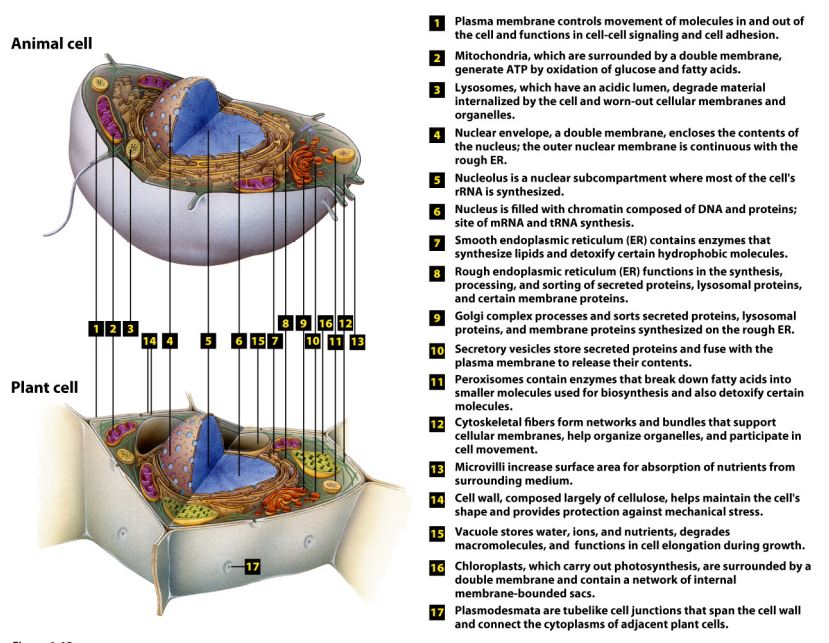
\includegraphics[width=1\textwidth]{images/schemagenerale.JPG}
        \caption{\small cellula animale e vegetale a confronto}
        \label{fig:mesh1}
    \end{figure}
    
\section{Organismi modello}
    Gli organismi modello sono utili per studiare aspetti umani per via delle similitudini a livello genetico nonostante diversità morfologica e dimensionale.
    \subsection{Saccharomyces cerevisiae}
        Il lievito \textit{budding yeast} (\textit{Saccharomyces cerevisiae}) è un organismo eucariote composto di una sola cellula. Proprio per questo motivo è stato ampiamente utilizzato come organismo modello e studiato a fondo. \\
        Il suo ciclo di vita consiste in una fase aploide e una fase diploide. Un altro motivo per il suo ampio utilizzo è proprio la velocità di duplicazione dovuta alla fase aploide che velocizza l'analisi in ricerca genetica. Risulta inoltre facile da manipolare e economicamente poco costoso. \\
        Il suo genoma è composto da circa 12.6 milioni di paia di basi (pb). Per dare un confronto, Escherichia coli ne possiede 4.6 milioni e il genoma umano oltre 3.2 miliardi. Possiede sequenze introniche e il meccanismo di espressione dei geni è simile a quella dell'uomo.
    
    \subsection{Chlamydomonas reinhardtii}
        L'alga unicellulare \textit{chlamydomonas reinhardtii} è "l'analogo vegetale" per il lievito visto nel paragrafo precedente. Contiene cloroplasti ed effettua la fotosintesi. Anche in questo caso, è un organismo facile da manipolare in vitro.
    
    \subsection{Caenorhabditis elegans}
        Il nematode \textit{Caenorhabditis elegans} è un organismo pluricellulare conosciuto anche come \textit{Roundworm}. Ha fornito la base per molti studi, in particolare per quelli che riguardano la morte cellulare programmata. Da adulto, ha un numero costante di cellule pari a 959.
        \subsubsection{Esperimento di Sulston}
            Salston studia lo sviluppo da embrione ad adulto, alla fine del processo il numero delle cellule è sempre costante a 959 e le cellule si dividono sempre allo stesso modo (la cellula x sarà sempre figlia della cellula X).\\
            Durante la vita dell'organismo si può osservare che vengono prodotte 131 cellule extra alle 959 le quali vanno incontro a morte cellulare programmata per lo sviluppo corretto del verme. Questi stessi geni sono conservati a livello evolutivo.
    
    \subsection{Evoluzione e geni comuni degli organismi modello}
        Ci sono aspetti della biologia che non permettono di essere studiati tramite organismo come il lievito. L'organismo che permette uno studio più vicino all'uomo è la scimmia (il 99\% il genoma umano è uguale a quella delle scimmie bonobo e scimpanzè).\\
        Osservando organismi evolutivamente più distanti come il topo si osservano fenomeni di \textit{sintenia}, ovvero osservando stretch di DNA dei due organismi si nota un'allineamento dei geni.\\
        Anche tra organismi modelli distanti come il moscerino della frutta e il topo si notano geni omologhi per lo sviluppo di porzioni corporee in posizioni e con funzioni simili.\\
        Il moscerino della frutta sottoposto a una mutagenesi eyeLess, ha consentito di individuare il gene umano che a livello embrionale concorre alla mancata formazione dell'iride per l'uomo.

\pagebreak